% \documentclass[paper=a4, fontsize=11pt]{scrartcl} % A4 paper and 11pt font size
\documentclass[11pt, a4paper]{book}
\usepackage[a4paper, total={5.5in, 8.75in}]{geometry}
\usepackage[T1]{fontenc} % Use 8-bit encoding that has 256 glyphs
\usepackage[utf8]{inputenc}
\usepackage{fourier} % Use the Adobe Utopia font for the document - comment this line to return to the LaTeX default
\usepackage{listings} % para insertar código con formato similar al editor
\usepackage[spanish, es-tabla]{babel} % Selecciona el español para palabras introducidas automáticamente, p.ej. "septiembre" en la fecha y especifica que se use la palabra Tabla en vez de Cuadro
\usepackage{url} % ,href} %para incluir URLs e hipervínculos dentro del texto (aunque hay que instalar href)
\usepackage{graphics,graphicx, float} %para incluir imágenes y colocarlas
\usepackage[gen]{eurosym} %para incluir el símbolo del euro
\usepackage{cite} %para incluir citas del archivo <nombre>.bib
\usepackage{enumerate}
\usepackage{hyperref}
\usepackage{graphicx}
\usepackage{adjustbox}
\usepackage{booktabs}

\usepackage{tabularx}
\newcolumntype{L}{>{\raggedright\arraybackslash}X}
\newcolumntype{R}{>{\raggedleft\arraybackslash}X}

\usepackage[table,xcdraw]{xcolor}
\hypersetup{
	colorlinks=true,	% false: boxed links; true: colored links
	linkcolor=black,	% color of internal links
	urlcolor=cyan,		% color of external links
}

\renewcommand{\familydefault}{\sfdefault}
\usepackage{fancyhdr} % Custom headers and footers
\pagestyle{fancyplain} % Makes all pages in the document conform to the custom headers and footers
\fancyhead[L]{} % Empty left header
\fancyhead[C]{} % Empty center header
\fancyhead[R]{Ángel Gómez Martín} % My name
\fancyfoot[L]{} % Empty left footer
\fancyfoot[C]{} % Empty center footer
\fancyfoot[R]{\thepage} % Page numbering for right footer
%\renewcommand{\headrulewidth}{0pt} % Remove header underlines
\renewcommand{\footrulewidth}{0pt} % Remove footer underlines
\setlength{\headheight}{13.6pt} % Customize the height of the header
\setlength{\parskip}{1ex}

\usepackage{titlesec, blindtext, color}
\definecolor{gray75}{gray}{0.75}
\newcommand{\hsp}{\hspace{20pt}}
\titleformat{\chapter}[hang]{\Huge\bfseries}{\thechapter\hsp\textcolor{gray75}{|}\hsp}{0pt}{\Huge\bfseries}
\setcounter{secnumdepth}{4}
\usepackage[Lenny]{fncychap}

\definecolor{gray97}{gray}{.97}
\definecolor{gray75}{gray}{.75}
\definecolor{gray45}{gray}{.45}
\definecolor{gray30}{gray}{.94}

\lstset{
	frame=Ltb,
    framerule=0.5pt,
    aboveskip=0.5cm,
    framextopmargin=3pt,
    framexbottommargin=3pt,
    framexleftmargin=0.1cm,
    framesep=0pt,
    rulesep=.4pt,
    backgroundcolor=\color{gray97},
    rulesepcolor=\color{black},
    stringstyle=\ttfamily,
    showstringspaces = false,
    basicstyle=\scriptsize\ttfamily,
    commentstyle=\color{gray45},
    keywordstyle=\bfseries,
    numbers=left,
    numbersep=6pt,
    numberstyle=\tiny,
    numberfirstline = false,
    breaklines=true,
}
 

\begin{document}
	\begin{titlepage}
\newlength{\centeroffset}
\setlength{\centeroffset}{-0.5\oddsidemargin}
\addtolength{\centeroffset}{0.5\evensidemargin}
\thispagestyle{empty}

\noindent\hspace*{\centeroffset}\begin{minipage}{\textwidth}

\centering
\includegraphics[width=0.9\textwidth]{logos/logo_ugr.jpg}\\[1.4cm]

\textsc{ \Large TRABAJO FIN DE MÁSTER\\[0.2cm]}
\textsc{ GRADO EN INGENIERÍA INFORMÁTICA}\\[1cm]

{\Huge\bfseries Matroos \\}
\noindent\rule[-1ex]{\textwidth}{3pt}\\[3.5ex]
{\large\bfseries Creación, configuración y despliegue de bots en \textit{Discord} }
\end{minipage}

\vspace{2.5cm}
\noindent\hspace*{\centeroffset}
\begin{minipage}{\textwidth}
\centering

\textbf{Autor}\\ {Ángel Gómez Martín}\\[2.5ex]
\textbf{Director}\\ {Juan Julián Merelo Guervós}\\[2cm]
\includegraphics[width=0.3\textwidth]{logos/etsiit_logo.png}\\[0.1cm]
\textsc{Escuela Técnica Superior de Ingenierías Informática y de Telecomunicación}\\
\textsc{---}\\
Granada, 7 de Julio de 2022
\end{minipage}
\end{titlepage}

	\thispagestyle{empty}

\begin{center}
{\large\bfseries Matroos \\ Creación, configuración y despliegue de bots en \textit{Discord}. }\\
\end{center}
\begin{center}
Ángel Gómez Martín\\
\end{center}

%\vspace{0.7cm}

\vspace{0.5cm}
\noindent{\textbf{Palabras clave}: software libre, \textit{Discord}, bot
\vspace{0.7cm}

\noindent{\textbf{Resumen}\\
	

\cleardoublepage

\begin{center}
{\large\bfseries Matroos \\ Creación, configuración y despliegue de bots en \textit{Discord}. }\\
\end{center}
\begin{center}
	Ángel Gómez Martín\\
\end{center}
\vspace{0.5cm}
\noindent{\textbf{Keywords}: \textit{open source}, \textit{Discord}, bot
\vspace{0.7cm}

\noindent{\textbf{Abstract}\\


\cleardoublepage

\thispagestyle{empty}

\noindent\rule[-1ex]{\textwidth}{2pt}\\[4.5ex]

D. \textbf{Juan Julián Merelo Guervós}, Profesor del Departamento de Arquitectura y Tecnología de Computadores de la Universidad de Granada.

\vspace{0.5cm}

\textbf{Informa:}

\vspace{0.5cm}

Que el presente trabajo, titulado \textit{\textbf{Matroos}},
ha sido realizado bajo mi supervisión por \textbf{Ángel Gómez Martín}, y autorizo la defensa de dicho trabajo ante el tribunal
que corresponda.

\vspace{0.5cm}

Y para que conste, expiden y firman el presente informe en Granada a Julio de 2022.

\vspace{1cm}

\textbf{El director: }

\vspace{5cm}

\noindent Fdo: Juan Julián Merelo Guervós



\chapter*{Agradecimientos}

A mi tutor, JJ, por ofrecerme su ayuda, conocimientos y acertados comentarios para la realización de este proyecto.

A mis padres, Elia y Ángel, por ser un pilar fundamental y por empujarme a seguir aprendiendo cosas nuevas y a superarme cada día.

A mi hermana Cristina, por apoyarme y echarme una mano siempre que lo he necesitado.

Y a Paula, por aguantarme más que nadie todo este tiempo.


	\newpage
	\tableofcontents

	\newpage
	\listoffigures

	\listoftables 
	\newpage

	\chapter{Introducción}

\textit{Discord}\cite{discord} es una aplicación de mensajería de uso tanto personal como en empresas. Es semejante a otras herramientas que se usan en ámbitos similares, como \textit{Slack}\cite{slack} o \textit{TeamSpeak}\cite{teamspeak}, y ofrece distintos servicios de comunicación, como mensajería instantánea, chat de voz e integración con bots y videojuegos.

Estos últimos elementos son bastante importantes, ya que la integración con videojuegos ha hecho que \textit{Discord} gane visibilidad en los últimos años; y la integración con bots ha hecho que la herramienta sea una herramienta mucho más interactiva que las otras mencionadas. Más información en el estado del arte.

En concreto, este proyecto se centra en los bots, que podrían definirse como herramientas que, haciendo uso de diferentes permisos, ayudan a automatizar tareas dentro de un servidor de \textit{Discord}. Las funciones de éstos son prácticamente ilimitadas, aunque las más populares son moderación de usuarios y mensajes, música, envío de contenido, noticias o encuestas.

Usuarios más avanzados (como por ejemplo, un administrador de sistemas, o alguien que controla distintos equipos) que quieren hacer uso de este software y de su sistema de bots se ven obligados a crear distintos bots muy específicos y en ocasiones poco reutilizables. Si bien se podrían programar comandos más específicos en un único bot, sería una tarea tediosa la reutilización entre diferentes ámbitos.

Incidiendo en el aspecto de la creación de bots forma más técnica, se observa que actualmente hay tres maneras de usar bots en \textit{Discord}:

\begin{itemize}
	\item \textbf{Usar bots ya existentes}. El bot ya se encuentra creado, configurado y desplegado, y solo es necesario agregarlo al servidor para poder disfrutar de sus funcionalidades.
	\item \textbf{Crear un bot a alto nivel}. Este caso es similar al anterior, ya que se trata de un bot genérico, que es configurable en cierta medida para cada servidor. Esta configuración se hace a través de algún tipo de herramienta (generalmente una aplicación web) que permite configurar los comandos deseados. Por otro lado, ya que están pensados para un público general, las posibilidades de configuración son escasas. Suelen tener algunas plantillas de comandos básicos, como temporizadores o respuestas automáticas.
	\item \textbf{Crear un bot a bajo nivel}. En este caso el bot se crea haciendo uso de las diferentes \textit{API} que ofrece \textit{Discord} para ello y la personalización es máxima. En cambio, es más tedioso, y requiere conocimientos extra que algunos usuarios pueden no tener (como programación). Además hay que tener en cuenta que el bot debe ser desplegado manualmente, por lo que requiere un esfuerzo extra.
\end{itemize}

Además, en el caso de que se quisieran desplegar distintos bots al mismo tiempo y administrarlos desde un mismo entorno, no sería posible, ya que cada uno de estos es una instancia distinta.

Por tanto, se pretende desarrollar un \textit{framework} para crear bots de \textit{Discord} configurables que sean capaces de conectar con diferentes sistemas. La principal motivación a la hora de desarrollar este sistema es encontrar la manera de centralizar la creación y la administración de bots de este tipo, además de resolver los diferentes problemas planteados:

\begin{itemize}
	\item Dificultad al crear bots con funcionalidades específicas.
	\item Poca configuración en aspectos más técnicos, como administración de sistemas.
	\item Dificultad de manejar el despliegue de distintos bots al mismo tiempo.
\end{itemize}

Es por tanto, un software pensado para usuarios mas avanzados, ya que los usuarios con menor conocimiento de las tareas administrativas sólo hacen uso de estos bots una vez ya desplegados a través de los servidores de \textit{Discord}.

	\chapter{Estado del arte}

En este capítulo se hace un repaso de las distintas soluciones que existen actualmente para la creación de bots de \textit{Discord} y la configuración de sus comandos.

\section{Contexto y definiciones previas}

Los bots actúan como un usuario más dentro de un servidor de \textit{Discord}. En cambio, debido a su naturaleza, deben ser agregados a los servidores por usuarios humanos. Se pueden crear infinidad de bots, por lo que han surgido páginas web (como \href{https://top.gg/}{top.gg} o \href{https://bots.ondiscord.xyz/}{Bots on Discord}) que permiten que los usuarios encuentren bots ya creados y desplegados listos para ser utilizados en sus servidores. Estos cuentan con funcionalidades específicas, por lo que no pueden modificarse por los usuarios.

Además de este tipo de bots y webs, han surgido otras plataformas que permiten que los usuarios creen y configuren sus propios bots. Estas son las que se desarrollan en este capítulo. A continuación se enumeran algunos conceptos que son interesantes conocer ya que se utilizan tanto en este capítulo como en el resto del documento.

Conceptos técnicos, que definen la manera en la que se estructuran, configuran y definen los bots:

\begin{itemize}
	\item \textbf{Comandos predefinidos}. Comandos cuya funcionalidad está ya definida (y por tanto programada) y no puede ser modificada por un usuario.
	\item \textbf{Comandos personalizados}. Comandos que se pueden crear a partir de comandos predefinidos que pueden utilizarse con distintos parámetros para modificar su comportamiento.
	\item \textbf{Comandos reutilizables}. Comandos personalizados que una vez configurados pueden utilizarse en distintos bots.
	\item \textbf{Despliegue de un bot}. Todas aquellas tareas y actividades que hacen que un bot se encuentre disponible para ser usado por usuarios.
	\item \textbf{Control del despliegue}. Capacidad de controlar y monitorizar el despliegue de bots en un sistema.
\end{itemize}

Conceptos relacionados con funcionalidades de \textit{Discord}:

\begin{itemize}
    \item \textbf{Comandos de moderación}. Comandos cuya funcionalidad se centra en la moderación de usuarios en los servidores de \textit{Discord}.
\end{itemize}

\section{Soluciones actuales}

Las soluciones actuales se podrían dividir en dos grupos, las herramientas \textit{no-code} y aquellas herramientas que hacen uso de programación. En ambas la interacción con el sistema se hace a través de una aplicación web y, además, suelen tener una apariencia muy similar, siendo las \textit{no-code} algo más complejas de usar. Las primeras se centran en usuarios con menor conocimiento técnico, abstrayendo todos los detalles de este tipo. En cambio, las segundas son utilizadas por aquellos usuarios con un conocimiento informático más amplio.

En las siguientes secciones se incluyen las herramientas con características más interesantes. Por otro lado, para cada herramienta se incluye una tabla como la siguiente, donde se resumen las características más importantes de cada una de ellas.

\FloatBarrier
\begin{table}[h]
    \centering
    \def\arraystretch{1.25}
    \begin{adjustbox}{max width=\textwidth}
    \begin{tabularx}{325px}{|l|L|}
    \hline
        \multicolumn{2}{|c|}{\textbf{Nombre de la herramienta}} \\ \hline
    \hline
        \textbf{Tipo de comandos} & El tipo de comandos que provee la herramienta, y la cantidad de comandos personalizados que se pueden crear. \\ \hline
        \textbf{Comandos reutilizables} & Si los comandos se pueden reutilizar entre bots o no. \\ \hline
        \textbf{Control del despliegue} & Si el usuario tiene control del despliegue del bot o no. \\ \hline
        \textbf{Número de bots} & La cantidad de bots que el usuario puede crear y configurar. \\ \hline
        \textbf{Experiencia} & La experiencia de usuario a la hora de utilizar las herramientas. \\ \hline
        \textbf{Personalización extra} & Si la herramienta permite una personalización más avanzada, y si es de pago o no. \\ \hline
        \textbf{Características} & Las funcionalidades configurables en los bots. \\ \hline
        \textbf{Logs} & Si permiten que los usuarios tengan acceso a los logs de los bots. \\ \hline
        \textbf{Premium} & Coste de los planes de pago de la herramienta. \\ \hline
    \end{tabularx}
    \end{adjustbox}
    \caption{Cuadro resumen de las características de una herramienta.}
\end{table}
\FloatBarrier

\subsection{Herramientas \textit{no-code}}

Estas herramientas permiten la creación de bots sin hacer uso de recursos de programación o similares. Cuentan con un repertorio de comandos predefinidos, de los cuales se pueden crear comandos personalizados modificando los parámetros de estos. Esto se hace a través de interfaces gráficas sencillas compuestas por formularios y otros elementos.

Por ejemplo, el comando predefinido más común sirve para enviar mensajes. A partir de este comando se pueden crear distintos comandos personalizados, cambiando la palabra clave que los usuarios deben introducir (en los canales de texto) para activar el comando y el mensaje que el bot debe enviar.

En general la mayoría tienen una serie de funcionalidades gratuitas, teniendo que suscribirse a un plan de pago mensual para obtener funcionalidades extra. Estas suscripciones suelen tener un coste aproximado de cinco dólares mensuales, pudiendo comprar suscripciones anuales o incluso de por vida y suelen ofrecer un repertorio de comandos más amplio, conexiones con redes sociales, estadísticas de uso e incluso \textit{logging}.

En la mayoría de casos estas plataformas cuentan con un único bot que se debe agregar al servidor de \textit{Discord} deseado. Esto implica que el uso de estos servicios no permite por tanto agregar varios bots con distintas funcionalidades a un mismo servidor. Si un usuario utiliza \textit{ProBot} (servicio que se explica en detalle a continuación), entonces el bot que proporciona \textit{ProBot} sólo podrá utilizarse una sola vez por servidor.

En ellas se puede observar también uno de los principales problemas ya mencionados, la muy reducida personalización y reutilización de los comandos. En estos sistemas no se puede crear un comando específico con una funcionalidad concreta, sino que se basan en funcionalidades predefinidas no reutilizables.

Estas funcionalidades predefinidas son en su mayoría de moderación de usuarios y envío de mensajes, y no se pueden reutilizar entre distintos bots. Además, debido a la estructura y arquitectura de estas plataformas, los usuarios no pueden ampliar el repertorio de comandos, teniendo que conformarse con los existentes.

\subsubsection{\textit{ProBot}}

\href{https://probot.io/}{\textit{ProBot}} es sin duda la más interesante de las herramientas \textit{no-code} debido a que permite crear ilimitados comandos personalizados, siendo la principal desventaja que estos comandos son predefinidos, y no se puede cambiar su funcionalidad. Los comandos predefinidos se centran en moderación y mensajes automáticos, por lo que las posibilidades no son muy amplias.

A favor de esta herramienta también destaca que es sencilla de utilizar, la interfaz web intenta imitar a la de \textit{Discord} y es intuitiva. Por contra, es bastante intrusiva la modalidad \textit{premium}, ya que muchas secciones sugieren la compra de esta modalidad. Además es imposible controlar el despliegue del bot, y no es posible reutilizar comandos.

Sus características son:

\FloatBarrier
\begin{table}[h]
    \centering
    \def\arraystretch{1.25}
    \begin{adjustbox}{max width=\textwidth}
    \begin{tabularx}{325px}{|l|L|}
    \hline
        \multicolumn{2}{|c|}{\textbf{\textit{ProBot}}} \\ \hline
    \hline
        \textbf{Tipo de comandos} & Predefinidos (ilimitados) \\ \hline
        \textbf{Comandos reutilizables} & No \\ \hline
        \textbf{Control del despliegue} & No \\ \hline
        \textbf{Número de bots} & 1, único \\ \hline
        \textbf{Experiencia} & Sencilla \\ \hline
        \textbf{Personalización extra} & Requiere \textit{premium} (mensualidades) \\ \hline
        \textbf{Características} & Moderación, estadísticas, mensajes automáticos, música \\ \hline
        \textbf{Logs} & No \\ \hline
        \textbf{Premium} & \$60 al año \\ \hline
    \end{tabularx}
    \end{adjustbox}
    \caption{Características de \textit{ProBot}.}
\end{table}
\FloatBarrier

\FloatBarrier
\begin{figure}[h]
	\centering
	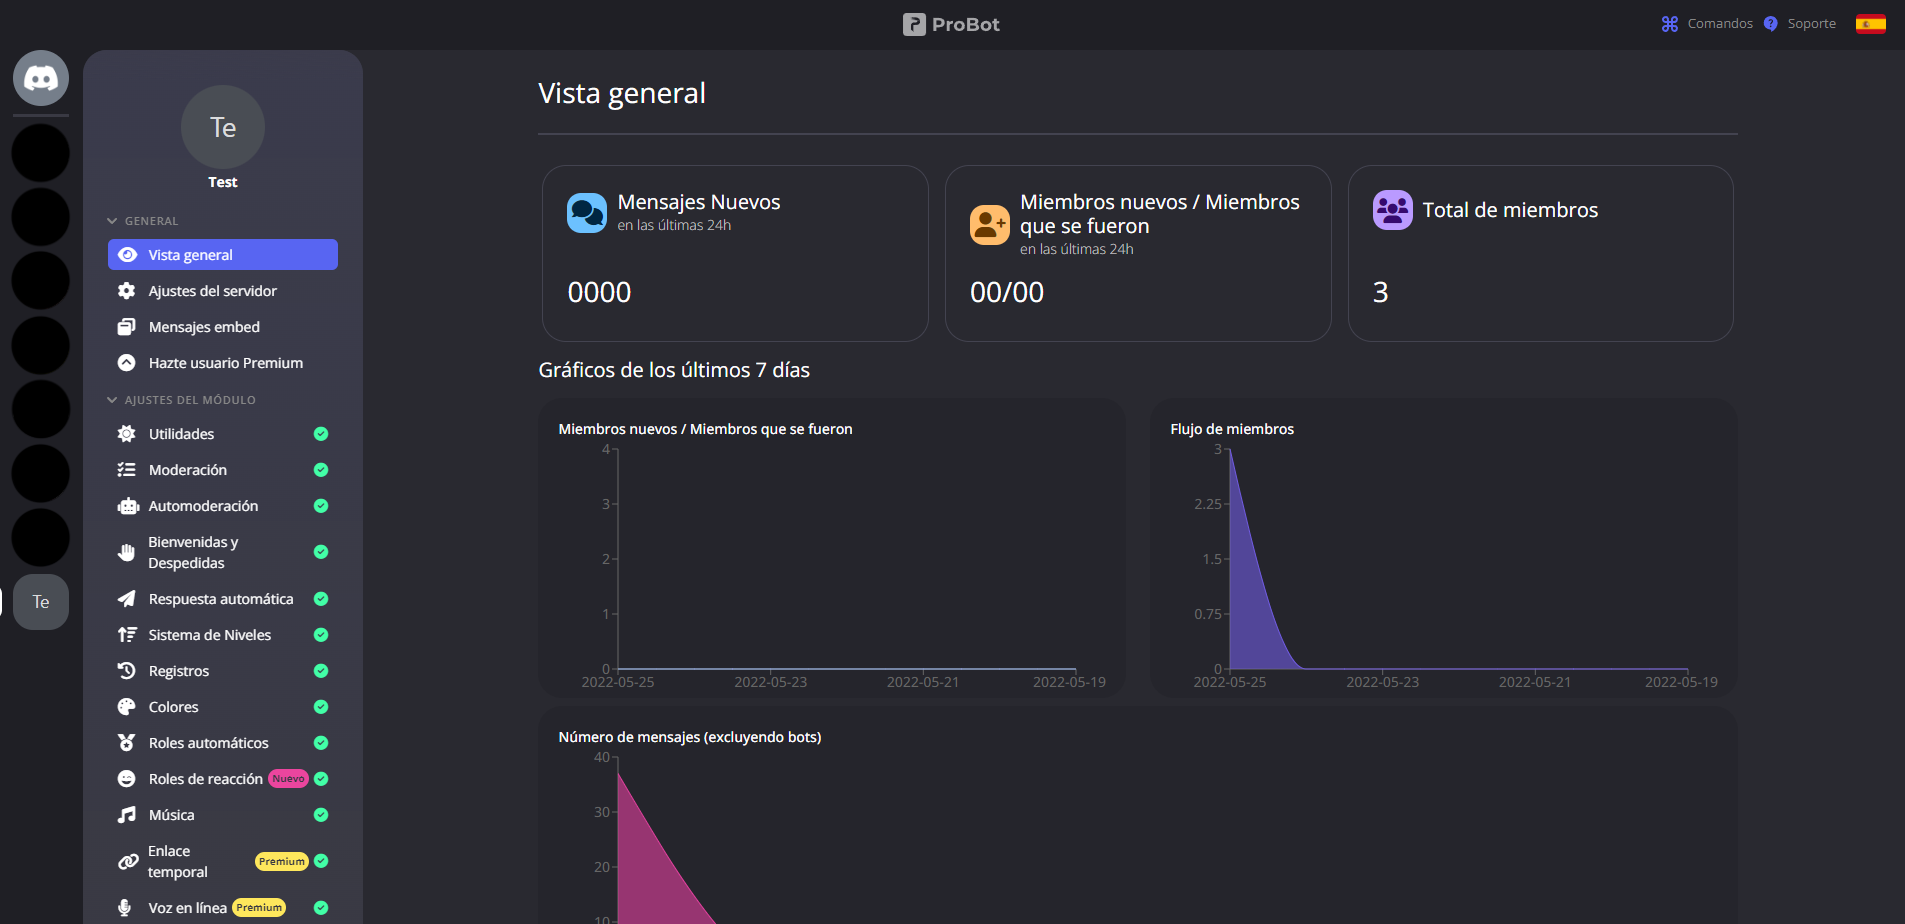
\includegraphics[width=1\textwidth]{img/probot.png}
	\caption{Interfaz web de \textit{ProBot}.}
\end{figure}
\FloatBarrier

\subsubsection{\textit{Mee6}}

\href{https://mee6.xyz/}{\textit{Mee6}} es otra herramienta muy similar a la anterior, siendo la principal diferencia que en este caso los comandos personalizados se limitan a 5. Por contra, tiene un mayor catálogo de funcionalidades.

De nuevo no es posible controlar el despliegue del bot, como tampoco es posible crear otro bot y agregarlo a un mismo servidor, o reutilizar comandos.

Sus características son:

\FloatBarrier
\begin{table}[h]
    \centering
    \def\arraystretch{1.25}
    \begin{adjustbox}{max width=\textwidth}
    \begin{tabularx}{325px}{|l|L|}
    \hline
        \multicolumn{2}{|c|}{\textbf{\textit{Mee6}}} \\ \hline
    \hline
        \textbf{Tipo de comandos} & Predefinidos (muy limitados, 5) \\ \hline
        \textbf{Comandos reutilizables} & No \\ \hline
        \textbf{Control del despliegue} & No \\ \hline
        \textbf{Número de bots} & 1, único \\ \hline
        \textbf{Experiencia} & Sencilla \\ \hline
        \textbf{Personalización extra} & Requiere \textit{premium} (mensualidades) \\ \hline
        \textbf{Características} & · Moderación, estadísticas, mensajes automáticos, música, temporizadores, \textit{quiz} / \textit{trivia} \\ \hline
        \textbf{Logs} & No \\ \hline
        \textbf{Premium} & \$50 al año / \$90 de por vida  \\ \hline
    \end{tabularx}
    \end{adjustbox}
    \caption{Características de \textit{Mee6}.}
\end{table}
\FloatBarrier

\FloatBarrier
\begin{figure}[h]
	\centering
	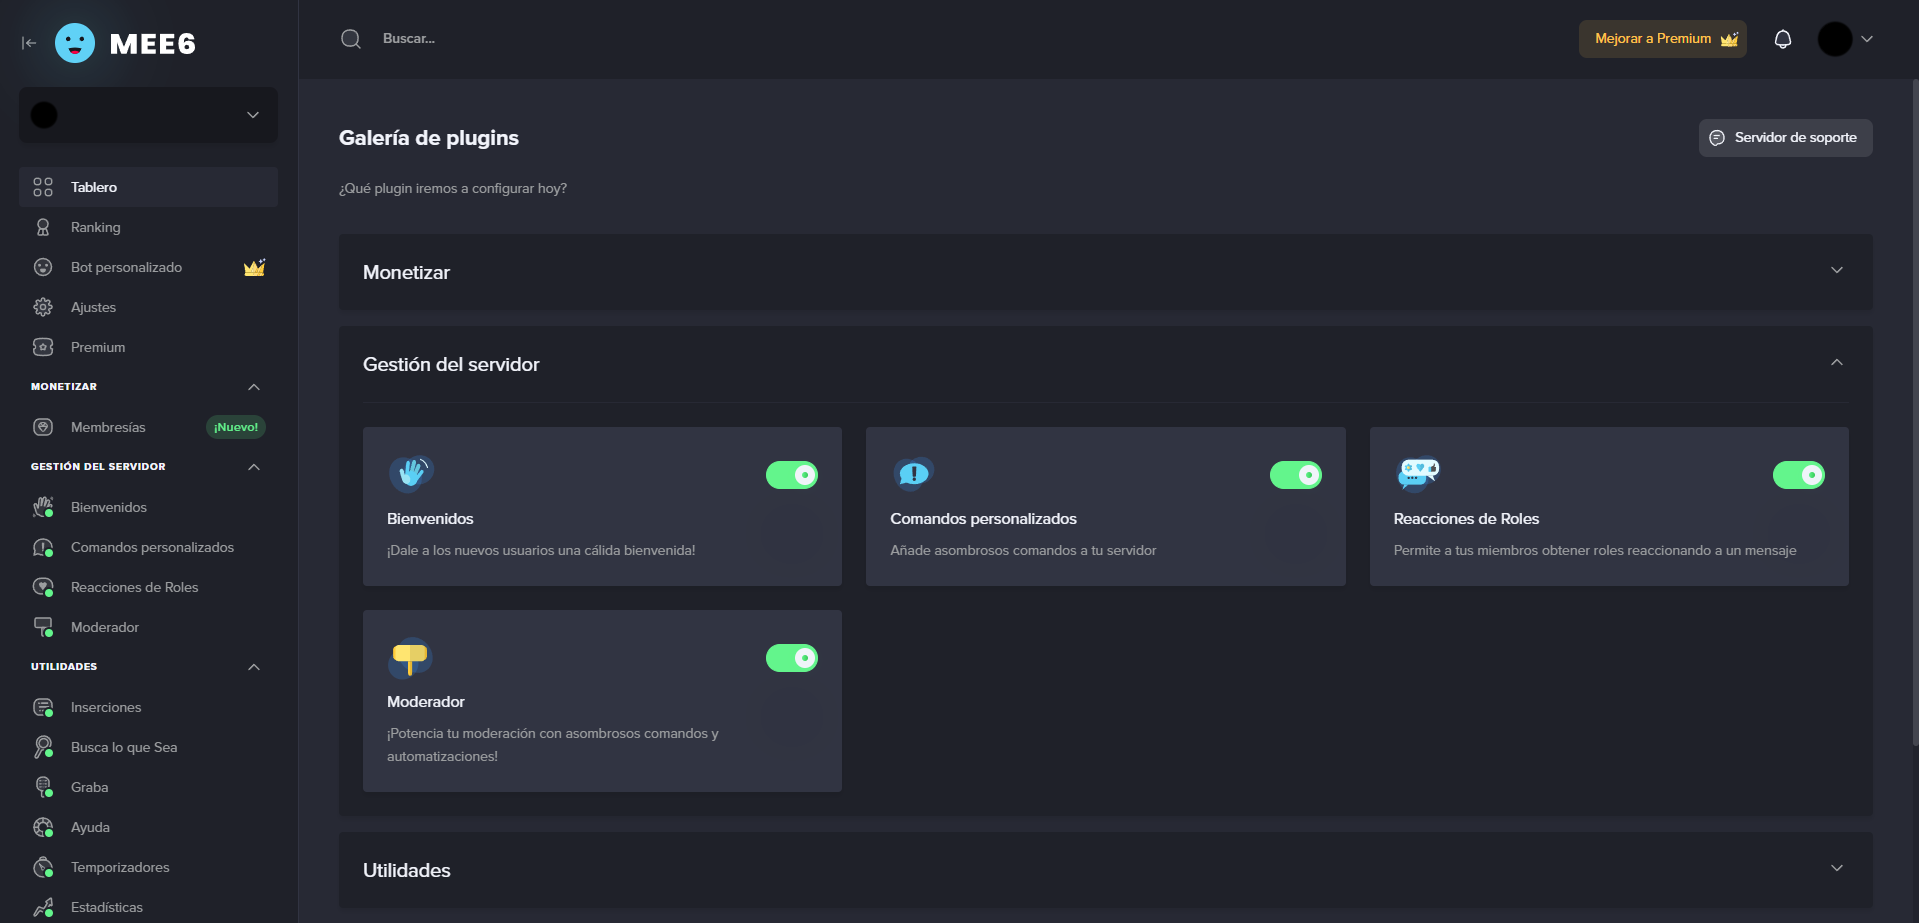
\includegraphics[width=1\textwidth]{img/mee6.png}
	\caption{Interfaz web de \textit{Mee6}.}
\end{figure}
\FloatBarrier


\subsubsection{\textit{BotGhost}}

\href{https://botghost.com/}{\textit{BotGhost}} es un híbrido entre \textit{ProBot} y \textit{Mee6}, ya que tiene características comunes de ambos. La principal característica de esta herramienta es que permite crear comandos personalizados haciendo uso de una serie de módulos que se pueden interconectar para definir el ciclo de vida de un comando.

Esta característica es muy interesante, pero está muy limitada y las funcionalidades que permite realizar se resumen en envío de mensajes y tareas de moderación de usuarios muy básicas. El plan \textit{premium} sería necesario en este caso para poder sacarle partido a esta funcionalidad.

Otro aspecto interesante es que se pueden crear distintos bots, hasta 50 distintos si se opta por la opción \textit{premium}. Sus características son las siguientes.

\FloatBarrier
\begin{table}[h]
    \centering
    \def\arraystretch{1.25}
    \begin{adjustbox}{max width=\textwidth}
    \begin{tabularx}{325px}{|l|L|}
    \hline
        \multicolumn{2}{|c|}{\textbf{\textit{BotGhost}}} \\ \hline
    \hline
        \textbf{Tipo de comandos} & Predefinidos (muy limitados, 5) \\ \hline
        \textbf{Comandos reutilizables} & Sí \\ \hline
        \textbf{Control del despliegue} & No (Sólo encendido y apagado) \\ \hline
        \textbf{Número de bots} & 1, único (50 con \textit{premium}) \\ \hline
        \textbf{Experiencia} & Compleja \\ \hline
        \textbf{Personalización extra} & Requiere \textit{premium} (mensualidades) \\ \hline
        \textbf{Características} & · Moderación, estadísticas, mensajes automáticos, temporizadores, integración con videojuegos, meteorología, música, \textit{quiz} / \textit{trivia} \\ \hline
        \textbf{Logs} & No \\ \hline
        \textbf{Premium} & \$60 al año / \$100 de por vida \\ \hline
    \end{tabularx}
    \end{adjustbox}
    \caption{Características de \textit{BotGhost}.}
\end{table}
\FloatBarrier

\FloatBarrier
\begin{figure}[h]
	\centering
	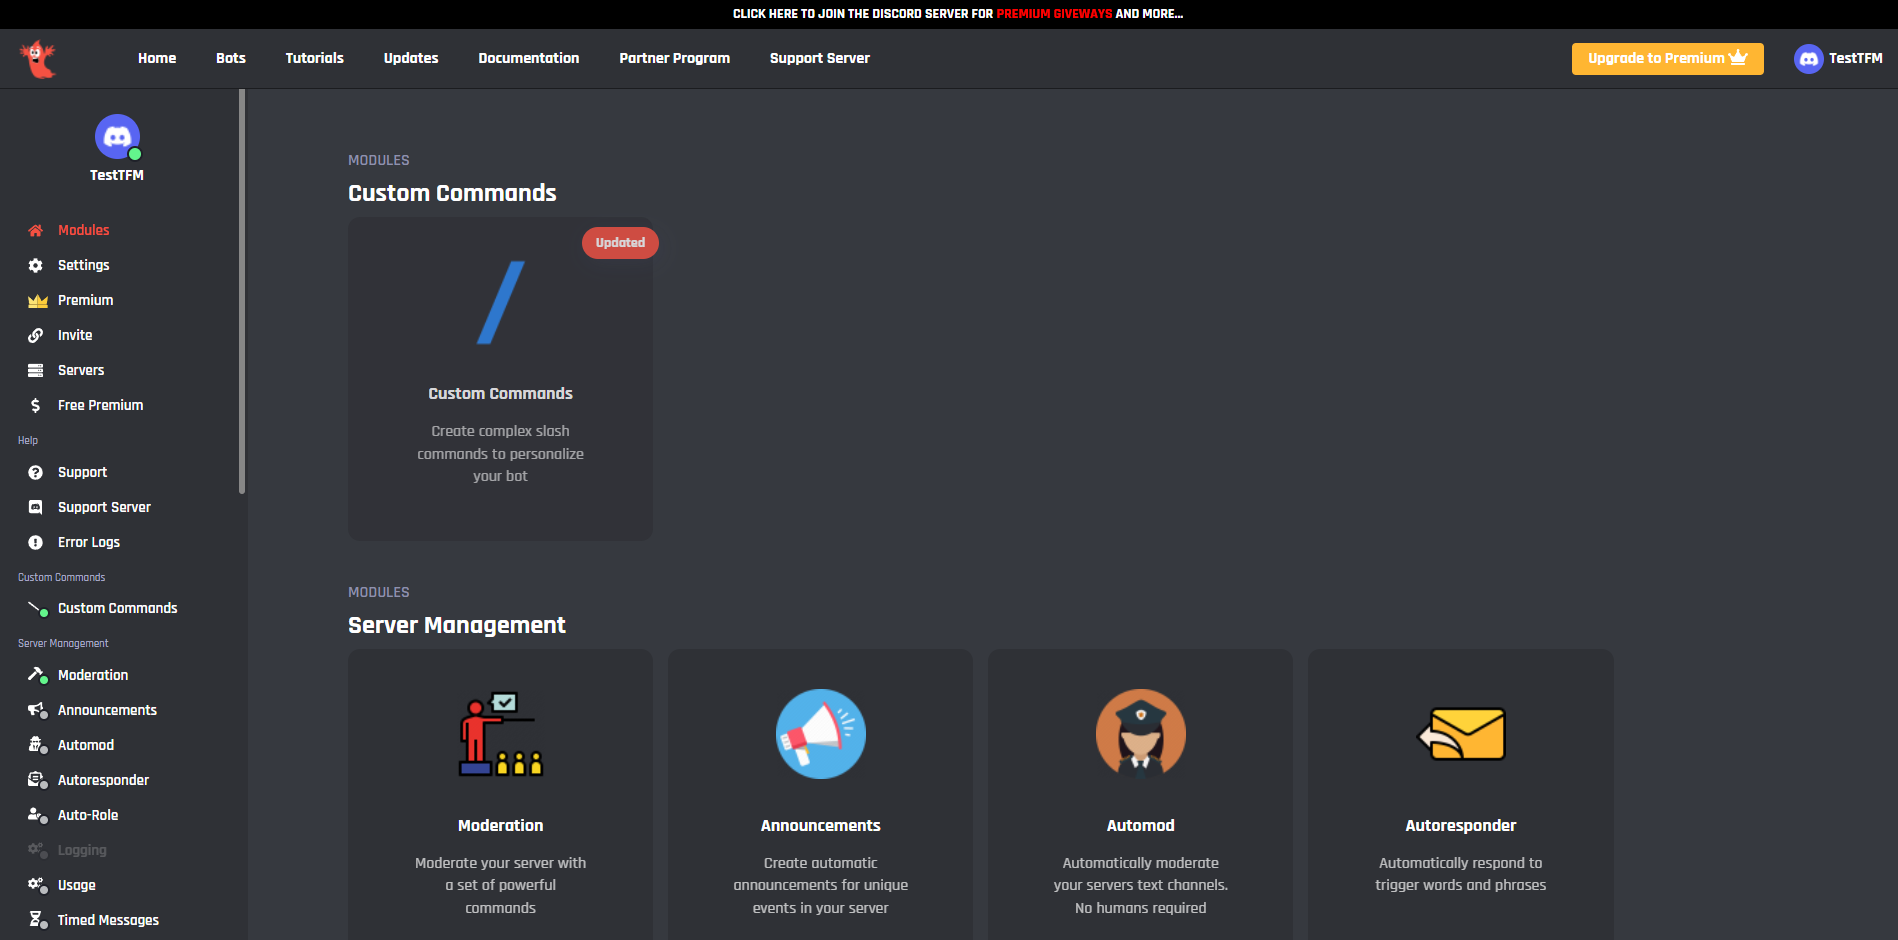
\includegraphics[width=1\textwidth]{img/botghost.png}
	\caption{Interfaz web de \textit{BotGhost}.}
\end{figure}
\FloatBarrier

\subsection{Herramientas de programación}

Actualmente existen multitud de librerías para distintos lenguajes de programación que permiten interactuar con la \textit{API} de \textit{Discord} y por tanto crear un bot. Así mismo existen herramientas híbridas que permiten esta creación de una manera más sencilla.

\subsubsection{\textit{Autocode}}

\href{https://autocode.com/}{\textit{Autocode}} es sin duda la herramienta mas interesante que existe de esta modalidad híbrida. Realmente es una plataforma que facilita la creación y despliegue de aplicaciones y servicios web, bots, y tareas de automatización permitiendo que los usuarios escriban sólo una parte del código (\textit{JavaScript}) de estos. Esta plataforma provee al usuario con un editor de código sencillo y de un explorador de archivos, recursos con los cuales puede crear el código.

De este modo el usuario sólo tiene que preocuparse por el código de la aplicación (o bot en este caso) que quiere crear, ya que del despliegue se encarga \textit{Autocode}. En su plan gratuito se pueden crear hasta 50 aplicaciones distintas, y permite la integración entre si de los distintos recursos que el usuario crea en la plataforma.

Sus características son:

\FloatBarrier
\begin{table}[h]
    \centering
    \def\arraystretch{1.25}
    \begin{adjustbox}{max width=\textwidth}
    \begin{tabularx}{325px}{|l|L|}
    \hline
        \multicolumn{2}{|c|}{\textbf{\textit{Autocode}}} \\ \hline
    \hline
        \textbf{Tipo de comandos} & Predefinidos + \textit{JS} \\ \hline
        \textbf{Comandos reutilizables} & No \\ \hline
        \textbf{Control del despliegue} & Sí (limitado) \\ \hline
        \textbf{Número de bots} & 50 gratis \\ \hline
        \textbf{Experiencia} & Algo complejo \\ \hline
        \textbf{Personalización extra} & Requiere \textit{premium} (mensualidades) \\ \hline
        \textbf{Especialidad} & Despliegue general de aplicaciones \\ \hline
        \textbf{Logs} & Sí (1-30 días) \\ \hline
        \textbf{Premium} & \$180 / \$1620 al año \\ \hline
    \end{tabularx}
    \end{adjustbox}
    \caption{Resumen de soluciones actuales.}
\end{table}
\FloatBarrier

\FloatBarrier
\begin{figure}[h]
	\centering
	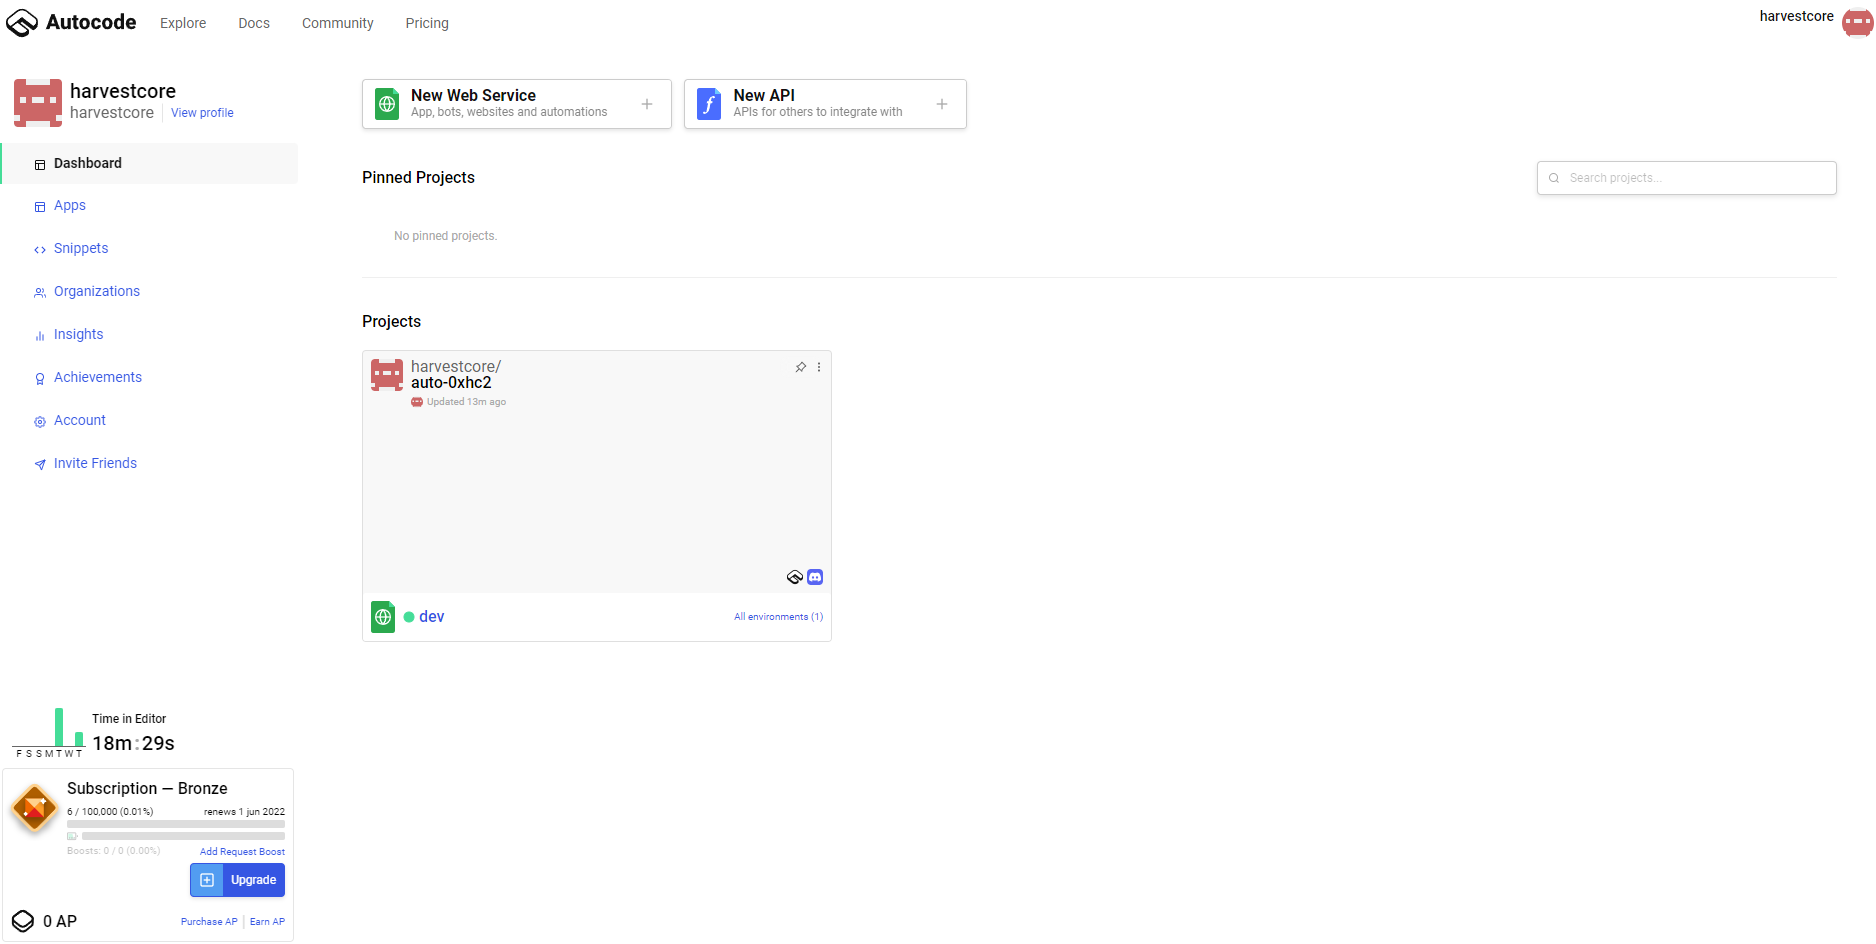
\includegraphics[width=1\textwidth]{img/autocode.png}
	\caption{Interfaz web de \textit{Autocode}.}
\end{figure}
\FloatBarrier

\subsubsection{Librerías de programación}

Las librerías de programación dan libertad total a la hora de crear un bot de \textit{Discord}, lo cual puede ser ideal en algunos casos. Las ventajas son obvias, ya que se puede crear cualquier tipo de comando y la reutilización es sencilla, pero en cambio, la gestión del despliegue puede ser compleja.

Por lo general todas las librerías permiten realizar casi las mismas funcionalidades, diferenciándose en aspectos como el rendimiento, la comunidad que las soporta o la facilidad de uso.

Algunos ejemplos de librerías son:

\begin{itemize}
	\item \textbf{\textit{C\#}}: \href{https://discordnet.dev/}{\textit{Discord.NET}}, \href{https://github.com/DSharpPlus/DSharpPlus}{\textit{DSharpPlus}}
	\item \textbf{\textit{Java}}: \href{https://github.com/DV8FromTheWorld/JDA}{\textit{JDA}}, \href{https://discord4j.com/}{\textit{Discord4J}}
	\item \textbf{\textit{C++}}: \href{https://dpp.dev/}{\textit{D++}}
	\item \textbf{\textit{JavaScript}}: \href{https://discord.js.org/}{\textit{discord.js}}
	\item \textbf{\textit{Golang}}: \href{https://github.com/bwmarrin/discordgo}{\textit{DiscordGo}}
	\item \textbf{\textit{Ruby}}: \href{https://github.com/shardlab/discordrb}{\textit{discordrb}}
\end{itemize}


\subsection{Comparativa de tiempos}

En esta sección se hace una comparativa del tiempo medio de desarrollo desde cero de un bot de \textit{Discord} usando las herramientas anterior mencionadas. Además se incluye tiempos de desarrollo usando tres lenguajes de programación: \textit{C\#}, \textit{JavaScript} y \textit{Python}.

Las mediciones incluyen todos los pasos necesarios para crear uno de estos bots con dos comandos personalizados. En el caso de las herramientas de programación se incluye desde la creación del proyecto hasta el despliegue (en local) de este.

Los dos comandos personalizados se han elegido al ser comunes en todas las plataformas mencionadas, además de sencillos de implementar. Son los siguientes:

\begin{itemize}
	\item Envío de un mensaje.
	\item Envío de un mensaje recurrente (cada cierto tiempo).
\end{itemize}

\FloatBarrier
\begin{table}[h]
    \centering
    \def\arraystretch{1.25}
    \begin{adjustbox}{max width=\textwidth}
    \begin{tabularx}{200px}{|l|R|}
    \hline
        \textbf{Herramienta} & \textbf{Tiempo (en minutos)} \\ \hline
    \hline
        ProBot & 5 \\ \hline
        Mee6 & 5 \\ \hline
        BotGhost & 10 \\ \hline
    \hline
        Autocode (JS) & 45 \\ \hline
    \hline
        JS & 85 \\ \hline
        C\# & 100 \\ \hline
        Python & 80 \\ \hline
    \end{tabularx}
    \end{adjustbox}
    \caption{Comparativa de tiempos de las distintas herramientas analizadas.}
\end{table}
\FloatBarrier

\section{Discusión}

Como se puede observar existen multitud de posibilidades a la hora de crear un bot de \textit{Discord}, y, aunque cumplen lo que prometen, se centran en aspectos muy concretos dejando otros bastante desatendidos.

En las herramientas \textit{no-code} los bots se centran principalmente en tareas de moderación, envío de mensajes, estadísticas e integración con videojuegos y redes sociales. Además, para sacarles partido es necesario el uso de los paquetes \textit{premium}, dejando de lado en el plan gratuito detalles específicos (y que serían ideales) como:

\begin{itemize}
	\item Reutilización de comandos.
	\item Creación de comandos con funcionalidad específica.
	\item Control del despliegue de los bots.
	\item Creación de distintos bots con distintas funcionalidades en un mismo sistema.
\end{itemize}

En el caso de las librerías de programación, aunque todas permiten el acceso a la \textit{API} de \textit{Discord}, cada una de ellas tiene una estructura distinta y los procedimientos para crear un bot o comandos son más o menos complejos. Si un usuario decidiese utilizarlas tendría flexibilidad completa a la hora de crear una estructura concreta, pero entonces tendría que dedicar en ese caso un tiempo necesario para diseñar algo funcional.

\textit{Autocode} es una buena alternativa a las soluciones anteriores, ya que se evita el tener que gestionar el despliegue de los bots y se eliminan algunas trabas de gestión del código, pero al igual que el uso de librerías toda la lógica recae en el usuario final. Esto puede ser útil en ciertos casos, pero no siempre.

En la comparativa de tiempos anterior se puede observar que las herramientas \textit{no-code} son las más rápidas. Esto se debe a que solo es necesario agregar el bot al servidor de \textit{Discord} deseado, y tras eso configurar de manera sencilla los comandos.

En menos de 10 minutos se puede incluir una gran cantidad de funcionalidad a un servidor de \textit{Discord} de manera gratuita, algo que puede ser muy útil para la basta mayoría de usuarios de \textit{Discord}, pero cuando se necesitan funcionalidades específicas entonces no es el sistema ideal.

En cambio, cuando se usan herramientas que hacen uso de código, el tiempo de implementación se incrementa considerablemente. No hace justicia la comparativa, ya que en este caso se tiene que desarrollar el software por completo, por lo que es obvio que el tiempo es mayor.

En definitiva, no existe ninguna herramienta sencilla que brinde lo mejor de ambas alternativas. Por un lado se quiere facilitar la creación de bots y comandos, y el despliegue de estos. Por otro se quiere poder ampliar el repertorio de comandos disponible de manera sencilla, sin tener que desarrollar una aplicación completa para ello.

	\chapter{Análisis}

En este capítulo se profundiza en el análisis del problema planteado en capítulos anteriores, describiendo las diferentes personas, historias de usuario y los \textit{user journeys} asociados a estas \textit{HU}.

\section{Personas}

\subsection{Administrador}
\label{sec:personaAdmin}

\begin{table}[H]
    \centering
    \def\arraystretch{1.25}
    \begin{adjustbox}{max width=\textwidth}
    \begin{tabularx}{\textwidth}{|l|L|}
    \hline
        \textbf{Nombre} & \textbf{David Infante} \\ \hline
    \hline
        Rol & Administrador \\ \hline
        Descripción & · 24 años.\linebreak · Disfruta de las tardes con sus amigos en \textit{Discord} jugando a sus videojuegos favoritos. \\ \hline
        Intereses & · \textit{Discord}, ya que le parece una herramienta muy potente.\linebreak · Videojuegos, le encantan los \textit{shooters}.\linebreak · Automatización de tareas repetitivas, ya que odia hacer lo mismo continuamente.\linebreak · Programación, ya que disfruta creando software para facilitar su día a día.\linebreak · Monitorización, le gusta saber que todo el software que despliega funciona correctamente.\linebreak · Creación de servidores de juegos, para jugar con sus amigos y no tener que depender de servidores de terceros. \\ \hline
        Formación & Ingeniero informático.\linebreak\linebreak Tiene conocimientos avanzados en:\linebreak · Configuración de \textit{Discord}.\linebreak · Administración de sistemas.\linebreak · Despliegue de software y sistemas. \\ \hline
        Frustraciones & Tener que realizar tareas repetitivas. \\ \hline
        Necesidades & Un software o sistema que le permita programar las tareas repetitivas de monitorización y automatización que tanto odia. Usa mucho \textit{Discord}, por lo que piensa que sería útil que el software estuviera integrado con esa herramienta. \\ \hline
    \end{tabularx}
    \end{adjustbox}
    \caption{Persona 1. Administrador.}
\end{table}


\subsection{Usuario de \textit{Discord}}
\label{sec:personaUsuarioDiscord}
\begin{table}[H]
    \centering
    \def\arraystretch{1.25}
    \begin{adjustbox}{max width=\textwidth}
    \begin{tabularx}{\textwidth}{|l|L|}
    \hline
        \textbf{Nombre} & \textbf{Jorge Pulido} \\ \hline
    \hline
        Rol & Usuario de \textit{Discord} \\ \hline
        Descripción & · 25 años.\linebreak · Amigo de Jorge Cancho. No tiene conocimientos de programación ni de temas relacionados con la ingeniería o la informática. Le gusta disfrutar de las tardes con sus amigos en \textit{Discord}. \\ \hline
        Intereses & · Videojuegos, dedica la mayor parte de su tiempo a jugar con sus amigos.\linebreak · La facilidad de las cosas, no le gusta complicarse la vida.\linebreak · \textit{Discord}, le parece una herramienta muy útil, ya que la usa con sus amigos y para temas laborales. \\ \hline
        Formación & Magisterio de educación primaria. \\ \hline
        Frustraciones & No le gusta nada tener que indagar en detalles técnicos al jugar a videojuegos con sus amigos. Entiende que en ocasiones es necesaria alguna configuración para poder jugar (como acceder a un servidor), pero quiere que ese proceso sea lo más fácil posible. No le gusta tener que recordar esos detalles, como la dirección del servidor al que acceder para jugar a ciertos juegos. \\ \hline
        Necesidades & Una herramienta que le permita acceder a esos detalles sin preocuparse de recordarlos o de consultarlos de manera extraña. Idealmente podría acceder a ellos a través de comandos de bots de \textit{Discord}. \\ \hline
    \end{tabularx}
    \end{adjustbox}
    \caption{Persona 2. Usuario de \textit{Discord}.}
\end{table}

\subsection{Miembro del tribunal}
\label{sec:personaMiembroTribunal}
\begin{table}[H]
    \centering
    \def\arraystretch{1.25}
    \begin{adjustbox}{max width=\textwidth}
    \begin{tabularx}{\textwidth}{|l|L|}
    \hline
        \textbf{Nombre} & \textbf{Blanca Casado} \\ \hline
    \hline
        Rol & Miembro del tribunal \\ \hline
        Descripción & · 52 años.\linebreak · Su conocimiento en informática es muy elevado, pero no tiene tanta destreza con las distintas aplicaciones de mensajería instantánea que han surgido en los últimos años. \\ \hline
        Intereses & · Procesamiento en segundo plano.\linebreak · Redes neuronales.\linebreak · Desarrollo ágil. \\ \hline
        Formación & Catedrática en informática. \\ \hline
        Frustraciones & No le gusta enfrentarse a documentaciones poco precisas o de dudosa credibilidad. \\ \hline
        Necesidades & Una documentación y una presentación acorde a los criterios de evaluación de TFM que le permita evaluar al estudiante. \\ \hline
    \end{tabularx}
    \end{adjustbox}
    \caption{Persona 3. Miembro del tribunal.}
\end{table}

\section{Historias de usuario}

Para la creación de las historias de usuarios se ha usado la siguiente estructura.

\begin{table}[H]
    \centering
    \def\arraystretch{1.25}
    \begin{adjustbox}{max width=\textwidth}
    \begin{tabularx}{\textwidth}{|l|L|}
    \hline
        \textbf{Sección} & \textbf{Significado} \\ \hline
    \hline
        Resumen & Breve resumen de la historia de usuario. \\ \hline
        Meta & Qué se quiere conseguir. \\ \hline
        Beneficio & El beneficio de la historia de usuario. \\ \hline
        Perfil de usuario & Perfil del usuario que genera la historia de usuario. \\ \hline
        Escenario & Escenario de la historia de usuario. Se deben especificar detalles más concretos.\linebreak · Dado …\linebreak · Cuando …\linebreak · Entonces … \\ \hline
        Dependencias & Posibles dependencias que tenga la historia de usuario. Éstas pueden ser otras historias de usuario, tareas que se estén llevando a cabo, etc. \\ \hline
        Tareas de seguimiento & Una vez analizada la historia de usuario, las tareas que se deben realizar a continuación. \\ \hline
        Criterio de aceptación & Criterio por el cual se va a determinar que la historia de usuario ha sido completada con éxito y por tanto finalizada. \\ \hline
    \end{tabularx}
    \end{adjustbox}
    \caption{Resumen historias de usuario.}
\end{table}

\bigskip

Por otro lado, se han creado las siguientes historias de usuario. Estas se encuentran en el \href{https://github.com/harvestcore/matroos}{repositorio} de \textit{GitHub} del proyecto, en la sección \href{https://github.com/harvestcore/matroos/labels/US}{\textit{Issues}}.

\begin{enumerate}
%	\item \href{https://github.com/harvestcore/matroos/issues/1}{Crear diferentes bots de \textit{Discord}}
	\item \textbf{Actualizar cuando las issues estén creadas en GitHub.}
\end{enumerate}


\subsection{HU-01 - Crear diferentes bots de \textit{Discord}}
\label{sec:hu01}

\begin{table}[H]
    \centering
    \def\arraystretch{1.25}
    \begin{adjustbox}{max width=\textwidth}
    \begin{tabularx}{\textwidth}{|l|L|}
    \hline
        \textbf{Sección} & \textbf{Contenido} \\ \hline
    \hline
        Resumen & Como usuario administrador quiero crear distintos bots de \textit{Discord} para poder separar funcionalidades en ellos. \\ \hline
        Meta & Creación de bots para separar funcionalidad en ellos. \\ \hline
        Beneficio & De este modo, cada bot puede tener una funcionalidad específica configurada, sin tener que compartir un bot con funcionalidades de distintos ámbitos. \\ \hline
        Perfil de usuario & \hyperref[sec:personaAdmin]{Administrador} \\ \hline
        Escenario & · Dado: que quiero crear distintos bots de \textit{Discord} y configurar sus funcionalidades,\linebreak · Cuando: proveo al sistema de los datos necesarios,\linebreak · Entonces: el sistema crea los bots para que pueda empezar a configurarlos. \\ \hline
        Tareas de seguimiento & \hyperref[sec:hu03]{HU-03}, \hyperref[sec:hu04]{HU-04}, \hyperref[sec:hu05]{HU-05}  \\ \hline
        Criterio de aceptación & · Los bots se pueden crear correctamente.\linebreak · El usuario es avisado en caso de error al crear un bot.\linebreak · Tests unitarios y integración son creados dentro de lo posible. \\ \hline
    \end{tabularx}
    \end{adjustbox}
    \caption{HU-01. Crear diferentes bots de \textit{Discord}.}
\end{table}


\subsection{HU-02 - Editar bots}
\label{sec:hu02}

\begin{table}[H]
    \centering
    \def\arraystretch{1.25}
    \begin{adjustbox}{max width=\textwidth}
    \begin{tabularx}{\textwidth}{|l|L|}
    \hline
        \textbf{Sección} & \textbf{Contenido} \\ \hline
    \hline
        Resumen & Como usuario administrador quiero poder cambiar la funcionalidad de los bots, ya que es posible que en ocasiones necesite ampliar o reducir sus comandos. \\ \hline
        Meta & Permitir agregar o eliminar comandos de los bots. \\ \hline
        Beneficio & Si quiero agregar nuevos comandos a un bot, o quitarlos, puedo hacerlo. \\ \hline
        Perfil de usuario & \hyperref[sec:personaAdmin]{Administrador} \\ \hline
        Escenario & · Dado: que quiero modificar los datos de los bots,\linebreak · Cuando: proveo al sistema de los datos que se quiero modificar,\linebreak · Entonces: el sistema modifica esos datos de los bots. \\ \hline
        Dependencias & \hyperref[sec:hu01]{HU-01} \\ \hline
        Tareas de seguimiento & – \\ \hline
        Criterio de aceptación & · El bot es modificado correctamente.\linebreak · El usuario es avisado en caso de error al modificar los datos del bot.\linebreak · Tests unitarios y integración son creados dentro de lo posible. \\ \hline
    \end{tabularx}
    \end{adjustbox}
    \caption{HU-02. Editar bots.}
\end{table}


\subsection{HU-03 - Repertorio de comandos ampliable}
\label{sec:hu03}

\begin{table}[H]
    \centering
    \def\arraystretch{1.25}
    \begin{adjustbox}{max width=\textwidth}
    \begin{tabularx}{\textwidth}{|l|L|}
    \hline
        \textbf{Sección} & \textbf{Contenido} \\ \hline
    \hline
        Resumen & Como usuario administrador quiero disponer de un repertorio de comandos predefinidos ampliable para después crear comandos personalizados a partir de ellos. \\ \hline
        Meta & Disponer de un repertorio de comandos predefinidos ampliable. \\ \hline
        Beneficio & De este modo, cuando se necesitan comandos predefinidos con funcionalidad nueva, es posible crearlos. \\ \hline
        Perfil de usuario & \hyperref[sec:personaAdmin]{Administrador} \\ \hline
        Escenario & · Dado: que quiero tener disponible una serie de comandos predefinidos,\linebreak · Cuando: necesito comandos con una funcionalidad nueva específica,\linebreak · Entonces: el sistema me permite implementarlos y utilizarlos más adelante. \\ \hline
        Dependencias & – \\ \hline
        Tareas de seguimiento & – \\ \hline
        Criterio de aceptación & · Los comandos predefinidos se pueden implementar correctamente.\linebreak · El usuario es avisado en caso de error al crear un comando.\linebreak · Tests unitarios y integración son creados dentro de lo posible. \\ \hline
    \end{tabularx}
    \end{adjustbox}
    \caption{HU-03. Repertorio de comandos ampliable.}
\end{table}

\subsection{HU-04 - Crear comandos personalizados}
\label{sec:hu04}

\begin{table}[H]
    \centering
    \def\arraystretch{1.25}
    \begin{adjustbox}{max width=\textwidth}
    \begin{tabularx}{\textwidth}{|l|L|}
    \hline
        \textbf{Sección} & \textbf{Contenido} \\ \hline
    \hline
        Resumen & Como usuario administrador quiero poder crear comandos personalizados a partir de los comandos predefinidos que se encuentran en el repertorio. \\ \hline
        Meta & La creación de comandos personalizados. \\ \hline
        Beneficio & Crear comandos personalizados con comportamientos concretos a partir de los comandos predefinidos existentes. \\ \hline
        Perfil de usuario & \hyperref[sec:personaAdmin]{Administrador} \\ \hline
        Escenario & · Dado: que quiero crear un comando personalizado,\linebreak · Cuando: proveo al sistema de los datos necesarios para crearlo,\linebreak · Entonces: el sistema crea el comando. \\ \hline
        Dependencias & \hyperref[sec:hu05]{HU-05} \\ \hline
        Tareas de seguimiento & \hyperref[sec:hu03]{HU-03} \\ \hline
        Criterio de aceptación & · El comando es modificado correctamente.\linebreak · El usuario es avisado en caso de error al modificar los datos del comando.\linebreak · Tests unitarios y integración son creados dentro de lo posible. \\ \hline
    \end{tabularx}
    \end{adjustbox}
    \caption{HU-04. Editar un comando.}
\end{table}

\subsection{HU-05 - Editar comandos personalizados}
\label{sec:hu05}

\begin{table}[H]
    \centering
    \def\arraystretch{1.25}
    \begin{adjustbox}{max width=\textwidth}
    \begin{tabularx}{\textwidth}{|l|L|}
    \hline
        \textbf{Sección} & \textbf{Contenido} \\ \hline
    \hline
        Resumen & Como usuario administrador quiero poder editar los detalles de un comando personalizado para cambiar su comportamiento y/o configuración. \\ \hline
        Meta & La edición de los parámetros de los comandos. \\ \hline
        Beneficio & Modificar la configuración de dicho comando. \\ \hline
        Perfil de usuario & \hyperref[sec:personaAdmin]{Administrador} \\ \hline
        Escenario & · Dado: que quiero modificar los datos de un comando,\linebreak · Cuando: proveo al sistema de los datos que quiero modificar,\linebreak · Entonces: el sistema modifica los datos del comando. \\ \hline
        Dependencias & \hyperref[sec:hu04]{HU-04} \\ \hline
        Tareas de seguimiento & – \\ \hline
        Criterio de aceptación & · El comando es modificado correctamente.\linebreak · El usuario es avisado en caso de error al modificar los datos del comando.\linebreak · Tests unitarios y integración son creados dentro de lo posible. \\ \hline
    \end{tabularx}
    \end{adjustbox}
    \caption{HU-05. Editar un comando.}
\end{table}

\subsection{HU-06 - Interfaz de usuario}
\label{sec:hu06}

\begin{table}[H]
    \centering
    \def\arraystretch{1.25}
    \begin{adjustbox}{max width=\textwidth}
    \begin{tabularx}{\textwidth}{|l|L|}
    \hline
        \textbf{Sección} & \textbf{Contenido} \\ \hline
    \hline
        Resumen & Como usuario administrador quiero disponer de una interfaz gráfica para poder realizar todas las gestiones del sistema de manera sencilla y visual. \\ \hline
        Meta & Disponer de una interfaz gráfica que permita realizar las tareas de creación, configuración y despliegue de bots de \textit{Discord}. \\ \hline
        Beneficio & Realizar todas las tareas de gestión de comandos y bots de manera sencilla en una interfaz de usuario, en lugar de hacerlas mediante el uso de una \textit{API}. \\ \hline
        Perfil de usuario & \hyperref[sec:personaAdmin]{Administrador} \\ \hline
        Escenario & · Dado: que quiero administrar los bots de \textit{Discord},\linebreak · Cuando: accedo a la interfaz gráfica,\linebreak · Entonces: el sistema me permite realizar todas las tareas de administración de bots y comandos. \\ \hline
        Dependencias & \hyperref[sec:hu01]{HU-01}, \hyperref[sec:hu02]{HU-02}, \hyperref[sec:hu03]{HU-03}, \hyperref[sec:hu04]{HU-04}, \hyperref[sec:hu05]{HU-05}, \hyperref[sec:hu06]{HU-06} \\ \hline
        Tareas de seguimiento & – \\ \hline
        Criterio de aceptación & · La interfaz permite realizar las tareas de gestión de bots y comandos.\linebreak · El usuario es avisado en caso de producirse algún error.\linebreak · Tests unitarios y integración son creados dentro de lo posible. \\ \hline
    \end{tabularx}
    \end{adjustbox}
    \caption{HU-06. Interfaz de usuario.}
\end{table}

\subsection{HU-07 - Criterios de evaluación}
\label{sec:hu07}

\begin{table}[H]
    \centering
    \def\arraystretch{1.25}
    \begin{adjustbox}{max width=\textwidth}
    \begin{tabularx}{\textwidth}{|l|L|}
    \hline
        \textbf{Sección} & \textbf{Contenido} \\ \hline
    \hline
        Resumen & Como miembro del tribunal, quisiera disponer de una documentación, una presentación y un informe acordes a los criterios de evaluación para comprobar que Estos se han cumplido correctamente. \\ \hline
        Meta & Disponer de una documentación que recoja claramente toda la información referente al desarrollo del TFM. \\ \hline
        Beneficio & De este modo es más sencillo evaluar todo el trabajo que el alumno ha realizado para desarrollar el TFM. \\ \hline
        Perfil de usuario & \hyperref[sec:personaMiembroTribunal]{Miembro del tribunal} \\ \hline
        Escenario & · Dado: que quiero evaluar el trabajo realizado por el alumno,\linebreak · Cuando: éste me de acceso a dicha documentación acorde a los criterios de evaluación,\linebreak · Entonces: podré evaluar el trabajo del alumno. \\ \hline
        Notas extra & Los criterios de evaluación son:\linebreak \linebreak El estudiante…\linebreak · Utiliza fuentes de información variadas, válidas y fiables y selecciona la relevante para el objetivo del trabajo.\linebreak · Toma decisiones adecuadas al contexto y propone soluciones utilizando el conocimiento adquirido.\linebreak · Detecta y analiza oportunidades para hacer nuevas propuestas.\linebreak · Propone soluciones adecuadas y justifica las decisiones tomadas para resolver problemas complejos.\linebreak · Utiliza recursos formales e informales para documentar adecuadamente el proceso de desarrollo: concepción, planificación, análisis, diseño, implementación, pruebas, etc.\linebreak · Muestra claridad y comprensión en la redacción,organizando la información adecuadamente y utilizando los recursos adecuados para el discurso escrito. Muestra claridad y comprensión en la expresión oral, organizando la información adecuadamente y utilizando los recursos adecuados para el discurso oral. \\ \hline
        Dependencias & – \\ \hline
        Tareas de seguimiento & – \\ \hline
        Criterio de aceptación & · La documentación cumple con los criterios de evaluación. \\ \hline
    \end{tabularx}
    \end{adjustbox}
    \caption{HU-07. Criterios de evaluación.}
\end{table}
  
\section{User journeys}

En esta sección se enumeran los \textit{user journeys} tanto para el uso del sistema, como para la ampliación del repertorio de comandos.

\subsection{Uso del sistema}

\subsubsection{Crear un bot}

\begin{enumerate}
	\item El usuario crea una aplicación de \textit{Discord} en el \href{https://discord.com/developers/applications}{portal de desarrolladores} y obtiene un \textit{token} para un bot.
	\item El usuario provee al sistema de este \textit{token} y de un nombre.
	\item[!] Si el nombre o el \textit{token} se encuentran en uso por otro bot, el sistema cancela la creación.
	\item El bot es creado en el sistema, quedando disponible para ser configurado con comandos o para ser desplegado.
\end{enumerate}

\subsubsection{Modificar un bot}

Se puede modificar un bot de dos maneras:

\begin{itemize}
	\item Parámetros del bot.
	\begin{enumerate}
		\item El usuario provee al sistema de datos del bot a actualizar.
		\item[!] Si los datos coinciden con los actuales o con los de otro bot, el sistema cancela la modificación.
		\item[!] Si el bot se encuentra desplegado, el sistema cancela el despliegue previa modificación.
		\item El sistema modifica los detalles del bot.
	\end{enumerate}
	
	\item Comandos del bot.
	\begin{enumerate}
		\item El usuario provee al sistema de los identificadores de los comandos personalizados que quiere agregar o eliminar del bot.
		\item[!] Si el bot se encuentra desplegado, el sistema cancela el despliegue previa modificación.
		\item El sistema modifica los comandos del bot.
	\end{enumerate}
\end{itemize}

\subsubsection{Eliminar un bot}

\begin{enumerate}
	\item El usuario provee al sistema del identificador del bot que quiere eliminar.
	\item[!] Si el bot se encuentra desplegado, el sistema cancela el despliegue previa eliminación.
	\item El sistema elimina todos los datos asociados al bot, no pudiendo volver a usarse.
\end{enumerate}

\subsubsection{Crear un comando personalizado}

\begin{enumerate}
	\item El usuario selecciona uno de los comandos predefinidos del repertorio.
	\item El usuario provee al sistema de los datos necesarios para crear un comando personalizado a partir del seleccionado.
	\item[!] Si los datos coinciden con los de otro comando, el sistema cancela la creación del comando.
	\item El sistema crea el comando.
\end{enumerate}

\subsubsection{Modificar un comando personalizado}

\begin{enumerate}
	\item El usuario provee al sistema de los datos que quiere modificar de un comando.
	\item[!] Si los datos que el usuario provee corresponden a otro comando, el sistema cancela la modificación.
	\item[!] Si el comando se encuentra en uso por un bot que se encuentra desplegado, el sistema cancela el despliegue previa modificación.
	\item El sistema modifica el comando.
\end{enumerate}

\subsubsection{Eliminar un comando personalizado}

\begin{enumerate}
	\item El usuario provee al sistema del identificador del comando que quiere eliminar.
	\item[!] Si el comando se encuentra en uso por un bot que se encuentra desplegado, el sistema cancela el despliegue previa eliminación.
	\item El sistema elimina todos los datos asociados al comando, no pudiendo volver a agregarse a un bot.
\end{enumerate}

\subsubsection{Desplegar un bot}

\begin{enumerate}
	\item El usuario provee al sistema del identificador del bot que quiere desplegar.
	\item[!] Si el bot ya se encuentra desplegado, el sistema cancela el despliegue.
	\item El sistema despliega el bot.
\end{enumerate}

\subsubsection{Cancelar despliegue de un bot}

\begin{enumerate}
	\item El usuario provee al sistema del identificador del bot del que quiere cancelar el despliegue.
	\item[!] Si el bot no se encuentra desplegado, el sistema cancela la operación.
	\item[!] Si el bot no existe, el sistema cancela la operación.
	\item El sistema cancela el despliegue del bot.
\end{enumerate}


\subsection{Ampliación del repertorio de comandos predefinidos}

Para la realización de este \textit{user journey} es necesario el uso de \textit{C\#}.

\begin{enumerate}
	\item El usuario define el nuevo tipo de comando.
	\item El usuario define los parámetros que necesita ese comando.
	\item El usuario implementa la funcionalidad asociada al comando, esto es el código que se ejecuta cuando el comando es invocado.
	\item El comando queda disponible para ser usado por el sistema.
	\item[!] Es necesario reiniciar el sistema para que pueda utilizarse el nuevo comando.
\end{enumerate}

\section{Modelo de negocio}

La solución propuesta se caracteriza por ser software libre, pero los costos de desarrollo e implementación nunca son nulos.

Debido a la muy probable falta de financiación al inicio del desarrollo del software, los objetivos iniciales se centrarían en obtener la renta mínima para poder continuar con el desarrollo del proyecto. A medida que se supere este primer obstáculo y el software esté mejor establecido, el modelo de financiación cambiaría para lograr un mayor valor de mercado y ganancias.

Como modelo de negocio, teniendo en cuenta que se opta por una solución compuesta por software libre, con el fin de sufragar todos estos gastos se podría optar por un modelo de consultoría. En este, se ofrecería soporte personalizado y desarrollo de características personalizadas para cada uno de los clientes que contratase el servicio. Otra posible fuente de ingresos podría ser el \textit{hosting} de bots mediante suscripciones mensuales, ofreciendo la herramienta y los bots como servicio.

\subsection{Sociedad Limitada Nueva Empresa}

Una \textit{SLNE} es una buena opción, ya que permite crear una pequeña empresa con pocos recursos iniciales con la que iniciar el desarrollo de forma profesional el desarrollo. Además tiene bastantes beneficios frente a otros modelos:

\begin{itemize}
	\item Construcción rápida.
	\item No necesita registro de socios.
	\item Fraccionado y aplazamiento de retenciones del \textit{IRPF} y otras deudas y pagos fraccionados.
	\item Se puede cambiar la denominación social de forma gratuita.
\end{itemize}

Los gastos para poder desarrollar un software de las características descritas de forma profesional no son desorbitados, pero tampoco son bajos. En cuanto a gastos derivados de la empresa y burocráticos serían (al menos) los siguientes:

\begin{itemize}
	\item 3000 euros. El capital mínimo a aportar para crear una \textit{SLNE}.
	\item 1000 euros. Estimación de los distintos gastos burocráticos.
	\item 550 euros. Gastos derivados con el desarrollo de la actividad laboral, como por ejemplo un local. Al año supone al menos 6600 euros.
\end{itemize}

Además, hay que tener en cuenta el salario del trabajador, que en este caso sería uno solo, para intentar abaratar costes. Los datos de empleo de 2022 en el sector de la Informática y Telecomunicaciones indican que el salario medio de una persona con aproximadamente 3 años de experiencia laboral (como es mi caso) se sitúa en 36500 euros brutos, lo que se traduce aproximadamente en 3050 euros brutos al mes. De nuevo, a fin de reducir los costes al inicio de la actividad laboral de esta empresa, se podría fijar un salario inferior, 28000 euros brutos al año.

A todas estas cifras habría que sumar todos los gastos relacionados con el desarrollo del software en sí, como pueden ser servicios de alojamiento del código, integración continua, copias de seguridad o sistemas y equipos informáticos. En una etapa inicial se podrían utilizar las versiones gratuitas de algunos estos servicios, pero en ciertos casos no sería posible ya que pueden ser necesarias otras características adicionales.

A continuación se muestra un posible presupuesto del gasto anual teniendo en cuenta todos los aspectos anterior mencionados.

\begin{table}[H]
    \centering
    \def\arraystretch{1.25}
    \begin{adjustbox}{max width=\textwidth}
    \begin{tabularx}{\textwidth}{|L|r|r|r|}
    \hline
        \textbf{Concepto} & \textbf{Euros/Ud} & \textbf{Cantidad} & \textbf{Total (Euros)} \\ \hline
    \hline
        Capital inicial (SLNE) & 3000 & 1 & 3000 \\ \hline
        Burocracia & 1000 & 1 & 1000 \\ \hline
        Derivados & 550 & 12 & 6600 \\ \hline
        Salario & 2333 & 12 & 28000 \\ \hline
        Servicios \textit{Cloud} & 150 & 12 & 1800 \\ \hline
        Sistemas informáticos & 3000 & 1 & 3000 \\ \hline
    \hline
        \multicolumn{3}{|r|}{\textbf{Total}} & \textbf{43400} \\ \hline
    \end{tabularx}
    \end{adjustbox}
    \caption{Presupuesto anual como \textit{SLNE}.}
\end{table}

Se puede observar que el primer año de vida de esta empresa (que hasta el momento sólo tiene un empleado) costaría más de 43000 euros, una cifra bastante alta. En el caso de que se quisiera incluir a un nuevo empleado, también desarrollador con experiencia similar, el coste adicional ascendería a aproximadamente 33000 euros.

\subsection{Autónomo}

Ser autónomo es otra posible opción para comenzar a desarrollar el software profesionalmente. En este caso los costes pueden ser algo inferiores, y además existen deducciones en el caso de ser una primera alta, pero no son bajos.

La siguiente tabla muestra el posible presupuesto del gasto anual:

\begin{table}[H]
    \centering
    \def\arraystretch{1.25}
    \begin{adjustbox}{max width=\textwidth}
    \begin{tabularx}{\textwidth}{|L|r|r|r|}
    \hline
        \textbf{Concepto} & \textbf{Euros/Ud} & \textbf{Cantidad} & \textbf{Total (Euros)} \\ \hline
    \hline
        Cuota mínima & 294 & 12 & 3528 \\ \hline
        Cuota máxima & 711 & 12 & 8532 \\ \hline
    \hline
        Burocracia & 1000 & 1 & 1000 \\ \hline
        Servicios \textit{Cloud} & 150 & 12 & 1800 \\ \hline
        Sistemas informáticos & 3000 & 1 & 3000 \\ \hline
    \hline
        \multicolumn{3}{|r|}{\textbf{Total (cuota mínima)}} & \textbf{9328} \\ \hline
        \multicolumn{3}{|r|}{\textbf{Total (cuota máxima)}} & \textbf{14332} \\ \hline
    \end{tabularx}
    \end{adjustbox}
    \caption{Presupuesto anual como \textit{autónomo}.}
\end{table}

Para este caso se ha mantenido el salario objetivo que se marcaba en la sección anterior, 28000 euros divididos en 12 pagas. Además, entra en juego la cuota de autónomos, que en 2022 sitúa su mínimo en 294 euros. Este aspecto es importante, ya que esta es la aportación por la que se cotiza. Si bien en los primeros meses podría ser interesante reducir al máximo los gastos, no es lo ideal a largo plazo. Otro aspecto importante es que se deberían pagar impuestos trimestrales, como el IVA, lo que incrementa los gastos.

	\chapter{Planificación}

\section{Metodología de desarrollo}
\label{sec:methodology}

La metodología de desarrollo se puede definir como el proceso disciplinado que busca ser eficiente a la hora de desarrollar un software. A lo largo del tiempo han surgido numerosas metodologías que buscan mejorarse unas a otras, haciendo hincapié en elementos como coste o calidad del desarrollo. De estas, destacan los principios ágiles, los cuales se usan en multitud de entornos laborales hoy en día.

Se ha utilizado \textit{GitHub} para la gestión de un repositorio para el código, además de para utilizar las herramientas que posee que facilitan el desarrollo del software.

Tras analizar el problema se han extraído una serie de casos de uso e historias de usuario, las cuales tienen especial importancia ya que de estas dependen las características del software final. En concreto, una vez establecidas las historias de usuario han surgido una serie de tareas, las cuales se han documentado en \textit{issues} en el \href{https://github.com/harvestcore/matroos}{repositorio}.

En el caso de este proyecto el desarrollo se ha dividido en diferentes hitos, los cuales están compuestos por las anteriores tareas e historias de usuario.

El proceso a seguir para el desarrollo es sencillo. Cuando es preciso trabajar en una tarea, se crea una rama de trabajo (usualmente nombrada con el identificador de la tarea, o un texto relevante). Sobre esta rama se publican una serie de \textit{commits} que solucionan el grueso de la tarea, y posteriormente se crea un \textit{pull request} (o \textit{PR}). Esta acción permite revisar lo que se quiere unir a la rama principal de desarrollo del software, con el fin de detectar errores o iniciar discusiones si fuese necesario.

\section{Temporización}

Como se menciona en la sección de \hyperref[sec:methodology]{metodología}, el trabajo se divide en \textit{hitos} de duración variable, ya que cada uno puede requerir mayor o menor cantidad de tiempo.

En total se han creado \href{https://github.com/harvestcore/matroos/issues}{67 issues}, habiéndose completado 59 del total. El desarrollo del proyecto comenzó a finales de febrero de 2022 y ha terminado a principios de Julio de 2022.

\section{PMV y Milestones}

Un producto mínimamente viable, o \textit{PMV}, es un producto con las suficientes características capaz de atraer a los posibles clientes o usuarios tan pronto como sea posible.

Para la realización de este proyecto se ha propuesto la creación de los siguientes \textit{PMV} (o \textit{milestones}, como se llaman en \href{https://github.com/harvestcore/matroos/milestones}{GitHub}).

Los \textit{milestones} 0 a 6 son los principales del proyecto, y son los que se planea inicialmente realizar. Los \textit{milestones} 8 y 9 son adicionales, y completarían el desarrollo de todo el software incluyendo funcionalidad y características extra.

\subsection{Milestones principales}

\subsubsection{00 - Configuración del entorno, tests y CI}

Enlace en \href{https://github.com/harvestcore/matroos/milestone/3}{GitHub}.

\textbf{Versión objetivo: 0.0.1}

El \textit{PMV} incluirá:

\begin{itemize}
	\item La estructura del repositorio está definida e implementada.
	\item Los proyectos necesarios están creados y listos para continuar con el desarrollo de nuevas funcionalidades.
	\item \textit{CI} está listo para ejecutar los diferentes tests y pruebas implementadas en los distintos proyectos.
	\item La documentación hasta este punto del desarrollo está actualizada y disponible.
\end{itemize}

Decisiones técnicas y documentación adicional:

\begin{itemize}
	\item Lenguaje de programación y \textit{framework}.
	\item Integración continua.
	\item Arquitectura.
\end{itemize}

\subsubsection{01 - Modelado del dominio del problema y lógica de negocio}

Enlace en \href{https://github.com/harvestcore/matroos/milestone/12}{GitHub}.

\textbf{Versión objetivo: 0.0.2}

El \textit{PMV} incluirá:

\begin{itemize}
	\item El dominio del problema está modelado.
	\item La lógica de negocio en su forma más básica está definida.
	\item La documentación hasta este punto del desarrollo está actualizada y disponible.
\end{itemize}

Decisiones técnicas y documentación adicional:

\begin{itemize}
	\item Arquitectura.
	\item Comandos.
	\item Bots.
	\item Herramientas.
\end{itemize}

\subsubsection{02 - Gestión de comandos}

Enlace en \href{https://github.com/harvestcore/matroos/milestone/10}{GitHub}.

\textbf{Versión objetivo: 0.0.3}

Tras la finalización de este \textit{milestone}:

\begin{itemize}
	\item La estructura de los comandos está definida.
	\item El \textit{backend} cuenta con un servicio capaz de gestionar los comandos y su configuración.
	\item Los tipos de comandos básicos quedan definidos y se pueden crear nuevos comandos de estos tipos.
	\item La documentación hasta este punto del desarrollo está actualizada y disponible.
\end{itemize}

Decisiones técnicas y documentación adicional:

\begin{itemize}
	\item Arquitectura.
	\item Comandos.
\end{itemize}

\subsubsection{03 - Gestión de bots}

Enlace en \href{https://github.com/harvestcore/matroos/milestone/6}{GitHub}.

\textbf{Versión objetivo: 0.0.4}


El \textit{PMV} incluirá:

\begin{itemize}
	\item La estructura de los bots está definida.
	\item El \textit{backend} cuenta con un servicio capaz de gestionar los bots y su configuración.
	\item Es posible asociar comandos a bots.
	\item La documentación hasta este punto del desarrollo está actualizada y disponible.
\end{itemize}

Decisiones técnicas y documentación adicional:

\begin{itemize}
	\item Arquitectura.
	\item Bots.
\end{itemize}

\subsubsection{04 - Despliegue de bots en \textit{workers}}

Enlace en \href{https://github.com/harvestcore/matroos/milestone/5}{GitHub}.

\textbf{Versión objetivo: 0.0.5}


El \textit{PMV} incluirá:

\begin{itemize}
	\item Es posible desplegar (ejecutar) bots en los \textit{workers}.
	\item El \textit{backend} es capaz de comunicarse con los distintos \textit{workers}.
	\item La documentación hasta este punto del desarrollo está actualizada y disponible.
\end{itemize}

Decisiones técnicas y documentación adicional:

\begin{itemize}
	\item Lenguaje de programación y \textit{framework}.
	\item Arquitectura.
\end{itemize}

\subsubsection{05 - API REST}

Enlace en \href{https://github.com/harvestcore/matroos/milestone/7}{GitHub}.

\textbf{Versión objetivo: 0.1.0}


El \textit{PMV} incluirá:

\begin{itemize}
	\item La \textit{API Rest} está definida y los \textit{endpoints} están documentados.
	\item Es posible realizar las tareas de administración de bots y comandos haciendo uso de la API.
	\item La documentación hasta este punto del desarrollo está actualizada y disponible.
\end{itemize}

Decisiones técnicas y documentación adicional:

\begin{itemize}
	\item Lenguaje de programación y \textit{framework}.
	\item Arquitectura.
\end{itemize}

\subsubsection{06 - Despliegue en contenedores Docker}

Enlace en \href{https://github.com/harvestcore/matroos/milestone/2}{GitHub}.

\textbf{Versión objetivo: 0.2.0}


El \textit{PMV} incluirá:

\begin{itemize}
	\item El software es distribuible mediante contenedores Docker.
	\item El archivo \textit{Dockerfile} para el microservicio del \textit{backend} está disponible.
	\item El archivo \textit{Dockerfile} para el microservicio del \textit{worker} está disponible.
	\item El archivo \textit{Docker Compose} para orquestar los microservicios está disponible.
	\item La documentación hasta este punto del desarrollo está actualizada y disponible.
\end{itemize}

Decisiones técnicas y documentación adicional:

\begin{itemize}
	\item Despliegue en contenedores.
	\item Arquitectura.
\end{itemize}

\subsubsection{07 - Almacén de datos}

Enlace en \href{https://github.com/harvestcore/matroos/milestone/11}{GitHub}.

\textbf{Versión objetivo: 0.3.0}


El \textit{PMV} incluirá:

\begin{itemize}
	\item Tanto los bots como los comandos son almacenables en base de datos.
	\item La documentación hasta este punto del desarrollo está actualizada y disponible.
\end{itemize}

Decisiones técnicas y documentación adicional:

\begin{itemize}
	\item Herramientas (Base de datos).
	\item Arquitectura.
	\item Base de datos.
\end{itemize}

\subsection{Milestones adicionales}

\subsubsection{08 - Interfaz de usuario}

Enlace en \href{https://github.com/harvestcore/matroos/milestone/9}{GitHub}.

\textbf{Versión objetivo: 0.4.0}


El \textit{PMV} incluirá:

\begin{itemize}
	\item La interfaz de usuario está disponible y es capaz de realizar las tareas de creación y configuración de comandos y bots, además del despliegue de éstos en \textit{workers}.
	\item La interfaz de usuario es distribuible mediante contenedores \textit{Docker}.
	\item El archivo \textit{Dockerfile} para el microservicio está disponible.
	\item La documentación hasta este punto del desarrollo está actualizada y disponible.
\end{itemize}

Decisiones técnicas y documentación adicional:

\begin{itemize}
	\item \textit{Frontend}.
	\item Arquitectura.
\end{itemize}

	\chapter{Herramientas y tecnologías utilizadas}
 

	\input{secciones/06_implementacion}
	\input{secciones/07_conclusiones}
	
	\newpage
	\bibliography{biblio}
	\bibliographystyle{plain}
	
\end{document}

